\documentclass[border=0cm]{standalone}
\input{john_macros}

\usepackage[T1]{fontenc}    % use 8-bit T1 fonts
\usepackage{graphicx}
\usepackage{overpic}
\usepackage{amsmath,amssymb}
%\usepackage{textcomp}
\usepackage[theoremfont]{newpxtext}
\usepackage{cabin}
%\usepackage[varqu,varl]{inconsolata}
\usepackage[bigdelims,vvarbb]{newpxmath}
%\usepackage[scr=boondoxo]{mathalfa}
\newcommand\hmmax{0}
\newcommand\bmmax{0}
\usepackage{bm}
\usepackage{mathrsfs}

\usepackage{pgfplots}
\usepackage{tikz}
\pgfplotsset{compat=newest}
\usepgfplotslibrary{fillbetween}
\usetikzlibrary{shapes.misc, shapes.geometric, arrows,
positioning, decorations.pathreplacing,calc,shadings}
\tikzstyle{line} = [draw, -latex']

\begin{document}


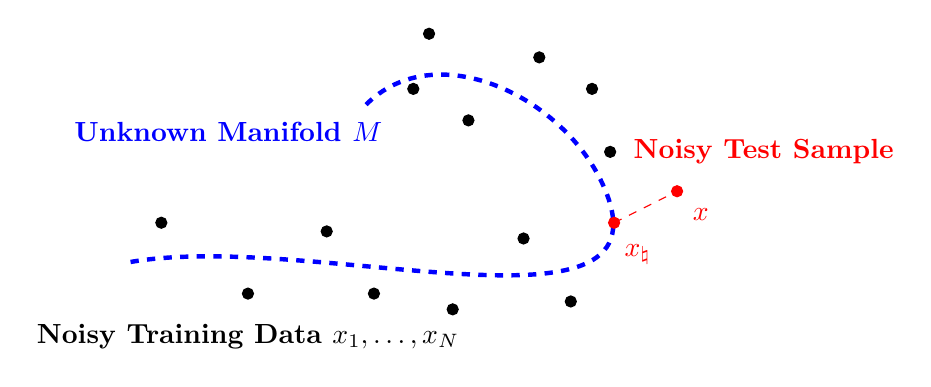
\begin{tikzpicture}
%\draw [blue, thick, xshift=4cm] plot [smooth, tension=2] coordinates { (0,0) (1.5,.5) (3.25,-1.5) (4,0)};    
\draw [ultra thick,blue, dashed] (-2,2) to[out=45,in=115] (1,1) to[out=-180+115,in=10] (-5,0);
\node at (-3.75,1.65) {\color{blue} \bf Unknown Manifold $\mc M$};
\filldraw (0,.3) circle (2pt);
\filldraw (-3.5,-.4) circle (2pt);
\filldraw (-2.5,.39) circle (2pt);
\filldraw (-1.9,-.4) circle (2pt);
\filldraw (-4.6,.5) circle (2pt);
\filldraw (-.9,-.6) circle (2pt);
\filldraw (.6,-.5) circle (2pt);
\filldraw (1.1,1.4) circle (2pt);
\filldraw (.87,2.2) circle (2pt);
\filldraw (.2,2.6) circle (2pt);
\filldraw (-.7,1.8) circle (2pt);
\filldraw (-1.4,2.2) circle (2pt);
\filldraw (-1.2,2.9) circle (2pt);
\filldraw [red] (1.15,.5) circle (2pt);
\node at (1.45,.1) {\color{red} $\mb x_\natural$};
\node at (-3.5,-.95) {\color{black} \bf Noisy Training Data $\mb x_1, \dots, \mb x_N$};
\filldraw [red] (1.95,.9) circle (2pt);
\node at (2.25,.6) {\color{red} $\mb x$};
\node at (3.05,1.4) {\color{red} \bf Noisy Test Sample}; 
\draw [dashed, red] (1.15,.5) -- (1.95,.9); 
\end{tikzpicture}


\end{document}

